%%%%%%%%%%%%%%%%%%%%%%%%%%%%%%%
%% Folie: BackUp             %%
%%%%%%%%%%%%%%%%%%%%%%%%%%%%%%%
\begin{frame}
    \frametitle{Backup slides}

\end{frame}
\clearpage

\begin{frame}
    \frametitle{Backup slides -- Training Setup}
    \vspace*{0.8cm}

Adam optimizer ($\beta_1 = 0.5, \beta_2 = 0.999$)

Learning rate: $0.0004$

Learning rate decay: On

Batch size: $10$

Iterations: $80000$

Model parameters: \newline $122.979, \quad 487.107, \quad 1.938.819, \quad 7.736.067, \quad  30.905.859$

\end{frame}
\clearpage

\begin{frame}
    \frametitle{Backup slides -- Norms on unit circle}
	\vspace*{1.25cm}
	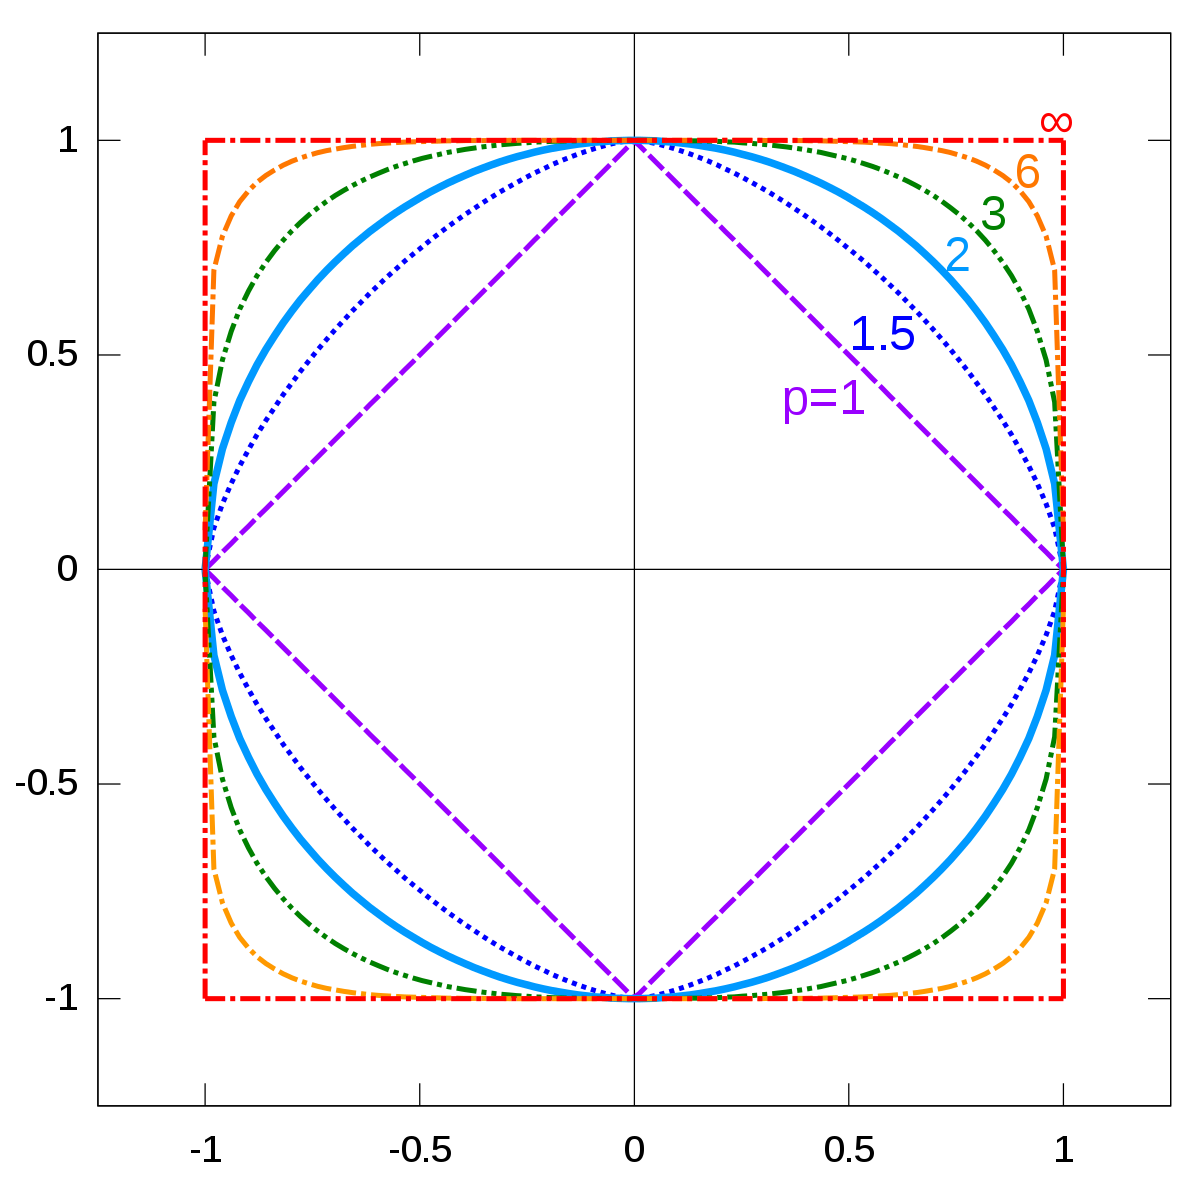
\includegraphics[width=0.3\textwidth, height=0.5\textheight]{./Ressourcen/Praesentation/Bilder/norms.png}

	Taken from: \url{https://de.wikipedia.org/wiki/Norm_(Mathematik)\#/media/Datei:Vector-p-Norms_qtl1.svg}

\end{frame}
\clearpage

\begin{frame}
    \frametitle{Backup slides -- Navier-Stokes}
\vspace*{0.8cm}

Navier-Stokes equation for incompressible flow:

$\frac{\partial u}{\partial t} + (u \cdot \nabla)u - \nu \nabla^2 u = - \nabla (\frac{p}{\rho_0}) + g$\newline

\begin{PraesentationAufzaehlung}
\item $u$: velocity
\item $p$: pressure
\item $\nu$: kinematic viscosity
\item $\rho_0$: uniform density
\item $g$: gravitational acceleration
\end{PraesentationAufzaehlung}

\end{frame}
\clearpage

\begin{frame}
    \frametitle{Backup slides -- Saint-Venant}
\vspace*{0.8cm}

Saint-Venant equations for incompressible flow (1D):

${\frac {\partial A}{\partial t}}+{\frac {\partial \left(Au\right)}{\partial x}}=0$\newline
${\frac {\partial u}{\partial t}}+u\,{\frac {\partial u}{\partial x}}+g\,{\frac {\partial \zeta }{\partial x}}=-{\frac {P}{A}}\,{\frac {\tau }{\rho }}$\newline

\begin{PraesentationAufzaehlung}
\item $x$: coordinate
\item $t$: time
\item $A(x,t)$: cross-sectional area of the flow at $x$
\item $u(x,t)$: flow velocity
\item $\zeta (x,t)$: free surface elevation
\item $\tau (x,t)$: wall shear stress along the wetted perimeter P(x,t) of the cross section at x
\item $\rho$: (constant) fluid density
\item $g$: gravitational acceleration
\end{PraesentationAufzaehlung}

\end{frame}
\clearpage

\begin{frame}
    \frametitle{Backup slides -- Previous work}
\vspace*{0.8cm}

Previous work done in the area of physics simulations with deep learning:

\begin{PraesentationAufzaehlung}
\item Accelerating Eulerian Fluid Simulation With Convolutional Networks \newline \url{https://arxiv.org/pdf/1607.03597.pdf}
\item tempoGAN: A Temporally Coherent, Volumetric GAN for Super-resolution Fluid Flow \newline \url{https://arxiv.org/pdf/1801.09710.pdf}
\item Deep Neural Networks for Data-Driven Turbulence Models \newline \url{https://arxiv.org/pdf/1806.04482.pdf}
\item Data-driven discretization: a method for systematic coarse graining of partial differential equations \newline \url{https://arxiv.org/pdf/1808.04930v1.pdf}
\item Hidden Fluid Mechanics: A Navier-Stokes Informed Deep Learning Framework for Assimilating Flow Visualization Data \newline \url{https://arxiv.org/pdf/1808.04327.pdf}
\end{PraesentationAufzaehlung}

\end{frame}
\clearpage